\subsection{Deadlocks}

Deadlocks happen when processes wait on each other,
this can be expressed as a cycle in a task dependency graph.

\begin{figure}[h]
    \centering
    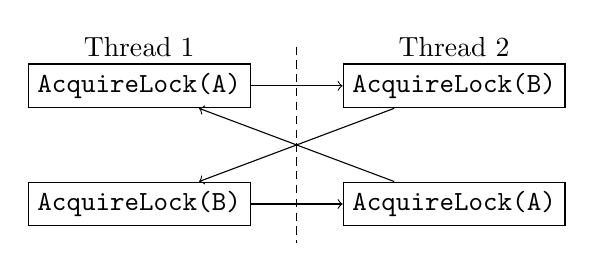
\begin{tikzpicture}
        % \draw (-2,-1) grid (2, 1);
        \node at (-2, 1.5) {Thread $1$};
        \node at (2, 1.5) {Thread $2$};
        \node [rectangle, draw, font=\ttfamily, name=th1_a] at (-2, 1) {AcquireLock(A)};
        \node [rectangle, draw, font=\ttfamily, name=th1_b] at (-2, -0.5) {AcquireLock(B)};
        \node [rectangle, draw, font=\ttfamily, name=th2_b] at (2, 1) {AcquireLock(B)};
        \node [rectangle, draw, font=\ttfamily, name=th2_a] at (2, -0.5) {AcquireLock(A)};
        \draw [->] (th1_a) -- (th2_b);
        \draw [->] (th1_b) -- (th2_a);
        \draw [->] (th2_a) -- (th1_a);
        \draw [->] (th2_b) -- (th1_b);
        \draw [densely dashed] (0, 1.5) -- (0, -1);
    \end{tikzpicture}
    \caption{Deadlock dependency graph.}
    \label{fig:deadlock}
\end{figure}

\subsubsection{System Model}
\begin{itemize}
    \item We have a finite number of resources.
    \item Resources are organized into classes.
    \item Processes compete for accessing resources.
    \item If a process requests an instance of a resource class,
    any instance of that class must satisfy the process.
\end{itemize}

\subsubsection{Resource Usage Protocol}
\begin{itemize}
    \item \textbf{Request} - the process either gets an instance of the resource immediately or waits until one is available.
    \item \textbf{Use} - the process can operate on its resource instance.
    \item \textbf{Release} - the process releases its resource instance.
\end{itemize}

\subsubsection{Deadlock Definition}
\paragraph{Informal Definition}
A set of two or more processes are deadlocked if:
\begin{itemize}
    \item They are blocked.
    \item Each is holding a resource.
    \item Each is waiting to acquire a resource held by another process in the set.
\end{itemize}
\paragraph{Formal Definition}
In a formal way the conditions necessary for a deadlock are the following:
\begin{itemize}
    \item \textbf{Mutual Exclusion} - only one process can use a resource at a time.
    \item \textbf{Hold \& Wait} - a process holding at least one resource is waiting to acquire additional resources which are currently held by other processes.
    \item \textbf{No Preemption} - a resource can only be released voluntarily by the process holding it.
    \item \textbf{Circular Wait} - a cycle of process requests exists ($P_0 \rightarrow P_1 \rightarrow \dots P_{n-1} \rightarrow P_0$).
\end{itemize}

\subsubsection{Deadlock Prevention}
Restrict the way requests can be made.

\paragraph{Mutual Exclusion}
Not required for shared resources, however it must hold for non-shareable files.

\paragraph{Hold \& Wait}
Must guarantee that whenever a process requests a resource, it does not hold any other resources.
Require the process to request and allocate all its resources before it begins execution.
Low resource utilization; possibly resulting in starvation.

\paragraph{No Preemption}
If a process that is holding some resources requests another resource that cannot be immediately allocated to it,
then all resources currently being held are released.
Preempted resources are added to the list of resources for which the process is waiting.
Process will be restarted only when it can regain its old resources, as well as the new ones that it is requesting.

\paragraph{Circular Wait}
Impose a total ordering of all resource types, requiring that each process requests resources in an increasing order of enumeration.

\subsubsection{Deadlock Avoidance}

Requires the system to have some additional \textit{à priori} information available.
\begin{itemize}
    \item Requires that each process declare the maximum number of resources of each type that it may need.
    \item The deadlock-avoidance algorithm dynamically examines the resource-allocation state to ensure that there can never be a circular-wait condition.
    \item Resource-allocation state is defined by the number of available and allocated resources and the maximum demands of the processes.
\end{itemize}

\paragraph{Banker's Algorithm}
In the banker's algorithm processes declare their maximum resource usage of each type of resource.
This number should not exceed the total number of resources in the system.
Whenever a process requests resources the system must determine if the allocation of such resources will leave the system in a safe state.
If it does leave the system in a safe state, the resources are allocated, otherwise the process must wait until enough resources are available.

Several data structures are required for the banker's algorithm,
these data structures encode the resource-allocation state.
In the following data structures, $n$ is the number of processes in the system and
$m$ is the number of resource types.
\begin{itemize}
    \item \textbf{Available} - A vector of length $m$ indicates the number of available resources of each type.
    If $\mathbf{Available}[j]$ equals $k$, then $k$ instances of resource type $R_i$ are available.
    \item \textbf{Max} - An $n \times m$ matrix defines the maximum demand of each process.
    If $\mathbf{Max}[i][j]$ equals $k$, then process $P_i$ may request at most $k$ instances of resource type $R_j$.
    \item \textbf{Allocation} - An $n \times m$ matrix defines the number of resources of each type currently allocated to each process.
    If $\mathbf{Allocation}[i][j]$ equals $k$, then process $P_i$ is currently allocated $k$ instances of resource type $R_j$
    \item \textbf{Need} - An $n \times m$ matrix indicates the remaining resource need of each process.
    If $\mathbf{Need}[i][j]$ equals $k$, then process $P_i$ may need $k$ more instances of resource type $R_j$ to complete its task.
    Note that $\mathbf{Need}[i][j] = \mathbf{Max}[i][j] - \mathbf{Allocation}[i][j]$.
\end{itemize}

The \textit{safety check} algorithm works as follows:
\begin{enumerate}
    \item Let \textbf{Work} and \textbf{Finish} be vectors of length $m$ and $n$, respectively.
    Initialize $\mathbf{Work} = \mathbf{Available}$ and $\mathbf{Finish} = false$ for $i = 0, 1, \dots, n - 1$.
    \item Find an index $i$ such that both:
    \begin{enumerate}
        \item $\mathbf{Finish}[i] == false$
        \item $\mathbf{Need}_i \le \mathbf{Work}$
    \end{enumerate}
    If no such $i$ exists, go to step 4.
    \item $\mathbf{Work} = \mathbf{Work} + \mathbf{Allocation}_i$\\
    $\mathbf{Finish}[i] = true$\\
    Go to step 2.
    \item If $\mathbf{Finish}[i] == true$ for all $i$, then the system is in a safe state.
\end{enumerate}

For the \textit{resource requesting} algorithm, let $\mathbf{Request}_i$ be the request vector for process $P_i$.
If $\mathbf{Request}_i [j] == k$, then process $P_i$ wants $k$ instances of resource type $R_j$.
The algorithm then works as follows:
\begin{enumerate}
    \item If $\mathbf{Request}_i \le \mathbf{Need}_i$, go to step 2.
    Otherwise, raise an error condition, since the process has exceeded its maximum claim.
    \item If $\mathbf{Request}_i \le \mathbf{Available}$, go to step 3.
    Otherwise, $P_i$ must wait, since the resources are not available.
    \item Have the system pretend to have allocated the requested resources to process $P_i$ by,
    modifying the state as follows:\\
    $\mathbf{Available} = \mathbf{Available} - \mathbf{Request}_i$\\
    $\mathbf{Allocation}_i = \mathbf{Allocation}_i + \mathbf{Request}_i$\\
    $\mathbf{Need}_i = \mathbf{Need}_i - \mathbf{Request}_i$\\
    If the resulting resource-allocation state if safe,
    the transaction is complete, and process $P_i$ is allocated its resources.
    However, if the new state is unsafe, then $P_i$ must wait for $\mathbf{Request}_i$,
    and the old resource-allocation state is restored.
\end{enumerate}
